\section{A catastrophe-aware population generating function}
\label{app:catastrophe-pgf}

We can retain population-count information without removing catastrophe from the model. For this purpose, use a killed, or defective, generating function. Its coefficients record the counts on paths that have not yet reached catastrophe. For $i=1,2$, define
\begin{subequations}
\label{eq:killed-pgf-definitions}
\begin{align}
\mathcal F_1(x,y,t)
&=\E_{(1,0)}
\!\left[x^{X_t}y^{Y_t}\boldsymbol 1_{\{\tau_{\!c}>t\}}\right],
\\
\mathcal F_2(x,y,t)
&=\E_{(0,1)}
\!\left[x^{X_t}y^{Y_t}\boldsymbol 1_{\{\tau_{\!c}>t\}}\right].
\end{align}
\end{subequations}
The variable $x$ plays no role in $\mathcal F_2$, but we keep both arguments so that the definitions remain parallel. We may also take the expectation over the catastrophe-free branching skeleton and write
\begin{equation*}
\mathcal F_i(x,y,t)
=\E_i\!\left[
x^{X_t}y^{Y_t}
\exp\!\left\{-\int_0^t
(\delta_1X_s+\delta_2Y_s)\,\dd s\right\}\right].
\end{equation*}
Hence,
\begin{equation*}
[x^my^n]\mathcal F_i(x,y,t)
=\Prob_i\{X_t=m,Y_t=n,\tau_{\!c}>t\},
\end{equation*}
and the total masses give the no-catastrophe probabilities:
\begin{equation*}
\mathcal F_1(1,1,t)=S(t),
\qquad
\mathcal F_2(1,1,t)=G(t).
\end{equation*}
Thus these functions are generally subnormalised at $(x,y)=(1,1)$. Their mass deficit is the probability that catastrophe has occurred by time $t$.

\begin{proposition}[Backward system for the killed generating functions]
\label{prop:killed-pgf-backward}
The functions in \cref{eq:killed-pgf-definitions} satisfy
\begin{subequations}
\label{eq:killed-pgf-backward}
\begin{align}
\partial_t\mathcal F_1
&=\lambda_1\mathcal F_1^2
-(\lambda_1+\mu_1+\nu+\delta_1)\mathcal F_1
+\mu_1+\nu\mathcal F_2,
\\
\partial_t\mathcal F_2
&=\lambda_2\mathcal F_2^2
-(\lambda_2+\mu_2+\delta_2)\mathcal F_2
+\mu_2,
\end{align}
\end{subequations}
with
\begin{equation}
\label{eq:killed-pgf-initial}
\mathcal F_1(x,y,0)=x,
\qquad
\mathcal F_2(x,y,0)=y.
\end{equation}
\end{proposition}

\begin{proof}
Condition on the first event, as in \cref{sec:model}. A birth produces two independent descendant lineages, which gives $\mathcal F_i^2$. Ordinary death leaves the empty population and contributes one, while conversion replaces $\mathcal F_1$ by $\mathcal F_2$. A catastrophe contributes zero. This last point explains why $\delta_i$ appears in the negative linear coefficient but not in the constant term: the catastrophe rate cannot be absorbed into the ordinary death rate.
\end{proof}

If $\delta_1=\delta_2=0$, \cref{eq:killed-pgf-backward,eq:killed-pgf-initial} becomes the Antal--Krapivsky generating-function system recovered in \cref{app:AK-recovery}. With positive catastrophe rates it is instead a Feynman--Kac deformation of that system, and its total mass need not equal one.

\subsection{The absorbing state and conditional populations}

To represent absorbed paths explicitly, let $\rho$ mark the absorbing state $\R$ and set
\begin{equation}
\label{eq:extended-pgf}
\mathcal H_i(x,y,\rho,t)
=\mathcal F_i(x,y,t)
+\rho\bigl[1-\mathcal F_i(1,1,t)\bigr].
\end{equation}
The coefficient of $\rho$ is the probability of catastrophe by time $t$. Hence,
\begin{equation*}
\mathcal H_i(1,1,1,t)=1.
\end{equation*}
Because the process stops at its first catastrophe, \cref{eq:extended-pgf} is linear in $\rho$. After absorption there is no finite pair of population counts.

On paths that avoid catastrophe up to time $t$, the population PGF is
\begin{equation}
\label{eq:conditional-pgf}
\mathcal Q_i(x,y,t)
=\frac{\mathcal F_i(x,y,t)}
{\mathcal F_i(1,1,t)}.
\end{equation}
For example, $\partial_x\mathcal Q_i(1,1,t)$ and $\partial_y\mathcal Q_i(1,1,t)$ are the conditional mean type-1 and type-2 counts. To record the population just before catastrophe, use the flux generating function
\begin{equation*}
\mathcal J_i(x,y,t)
=\delta_1x\,\partial_x\mathcal F_i(x,y,t)
+\delta_2y\,\partial_y\mathcal F_i(x,y,t).
\end{equation*}
This follows coefficientwise:
\begin{equation*}
[x^my^n]\mathcal J_i
=(\delta_1m+\delta_2n)
\Prob_i\{X_t=m,Y_t=n,\tau_{\!c}>t\},
\end{equation*}
the right-hand side is the time density of catastrophe from the pre-absorption state $(m,n)$. Summing over all counts gives
\begin{equation*}
\mathcal J_1(1,1,t)=-S'(t),
\qquad
\mathcal J_2(1,1,t)=-G'(t).
\end{equation*}

\subsection{Reuse of the hypergeometric solution}

The full killed PGF requires no new differential equation. We first rescale time:
\[
\widehat{\mathcal F}_i(x,y,\hat t)
=\mathcal F_i(x,y,\hat t/\lambda_1)
\]
and keep the notation $r_{2,\pm}$, $\alpha_2$, $\hat q_2$, $h$, and $A,B,C$ from \cref{sec:autonomous,sec:main_result}. In the generic regime of \cref{tt:thm:main}, only the starting coordinate changes:
\begin{equation}
\label{eq:pgf-z-coordinate}
z_{2,0}(y)=\frac{y-r_{2,-}}{y-r_{2,+}},
\qquad
z_2(\hat t;y)=z_{2,0}(y)\e^{\hat q_2\hat t}.
\end{equation}
Then the autonomous solution is
\begin{equation}
\label{eq:pgf-F2-solution}
\widehat{\mathcal F}_2(x,y,\hat t)
=r_{2,-}-\alpha_2
\frac{z_2(\hat t;y)}{1-z_2(\hat t;y)}.
\end{equation}

Suppose $z_{2,0}(y)\neq0$. Let $W_1,W_2$ be a fundamental pair of the Gauss equation \eqref{eq:hypergeometric}, chosen consistently along the path in \cref{eq:pgf-z-coordinate}. Write
\begin{equation*}
L(x,y)=\frac{h-x}{\hat q_2z_{2,0}(y)}
\end{equation*}
and define
\begin{align*}
K_1(x,y)
&=W_2'(z_{2,0}(y))
-L(x,y)W_2(z_{2,0}(y)),\\
K_2(x,y)
&=L(x,y)W_1(z_{2,0}(y))
-W_1'(z_{2,0}(y)).
\end{align*}
Then, with $z=z_2(\hat t;y)$,
\begin{equation}
\boxed{
\widehat{\mathcal F}_1(x,y,\hat t)
=h-\hat q_2z
\frac{K_1W_1'(z)+K_2W_2'(z)}
{K_1W_1(z)+K_2W_2(z)}.}
\label{eq:pgf-F1-solution}
\end{equation}
The Wronskian calculation in \cref{eq:K-coefficients} ensures that $\widehat{\mathcal F}_1(x,y,0)=x$. When $y=1$, the trajectory follows the negative real path used in the main theorem, so we may take $(W_1,W_2)=(U,V)$. Then \cref{eq:pgf-F1-solution,eq:pgf-F2-solution} reduce to $S$ and $G$ at $x=y=1$.

The exceptional value $z_{2,0}(y)=0$ follows by continuity. It can also be obtained directly because the type-2 solution is then constant. Extracting every coefficient with a bivariate Cauchy integral requires complex $x$ and $y$, so the second hypergeometric solution must use a consistent complex branch. One can avoid this branch choice by integrating \cref{eq:killed-pgf-backward} directly on the contour. Derivatives at $(x,y)=(1,1)$, including the conditional moments, stay on the original real branch.

\subsection{Three distributions encoded by the killed PGF}
\label{sec:three-pgf-distributions}

To keep the formulas readable, write
\begin{equation*}
p_{m,n}^{(i)}(t)
=[x^my^n]\mathcal F_i(x,y,t),
\qquad
\sigma_i(t)=\mathcal F_i(1,1,t),
\end{equation*}
so that $\sigma_1=S$ and $\sigma_2=G$. Normalising these coefficients gives the three distributions below.

\paragraph{Counts immediately before catastrophe.}
Once catastrophe occurs, the process enters the cemetery state $\R$. The counts of interest are therefore the left limits $(X_{\tau_{\!c}-},Y_{\tau_{\!c}-})$. Define
\begin{equation*}
j_{m,n}^{(i)}(t)
=(\delta_1m+\delta_2n)p_{m,n}^{(i)}(t).
\end{equation*}
From state $(m,n)$, catastrophe occurs at rate $\delta_1m+\delta_2n$. Thus $j_{m,n}^{(i)}(t)$ is the joint density of the catastrophe time and the state just before it. Conditional on catastrophe at time $t$, in the density sense, the PGF is
\begin{equation*}
\mathcal R_i(x,y\mid t)
=\frac{\mathcal J_i(x,y,t)}
{\mathcal J_i(1,1,t)},
\end{equation*}
and hence
\begin{equation*}
\Prob_i\{X_{\tau_{\!c}-}=m,Y_{\tau_{\!c}-}=n
\mid\tau_{\!c}=t\}
=\frac{j_{m,n}^{(i)}(t)}
{\mathcal J_i(1,1,t)}.
\end{equation*}
If we disregard the exact catastrophe time, the distribution conditional on catastrophe by a horizon $T$ has PGF
\begin{equation*}
\mathcal R_{i,T}^{\mathrm{cat}}(x,y)
=\frac{\displaystyle\int_0^T
\mathcal J_i(x,y,t)\,\dd t}
{1-\sigma_i(T)}.
\end{equation*}
As $T\to\infty$, this becomes the population distribution at eventual catastrophe, conditional on catastrophe occurring. Integrating the flux over all future times and assigning the forever-avoidance mass to the origin produces the unconditional ultimate release law of \cref{sec:ultimate-release}.

\paragraph{Counts given no catastrophe.}
At a fixed time $t$, \cref{eq:conditional-pgf} gives
\begin{equation*}
\Prob_i\{X_t=m,Y_t=n\mid\tau_{\!c}>t\}
=\frac{p_{m,n}^{(i)}(t)}{\sigma_i(t)}.
\end{equation*}
Ordinarily extinct paths remain in this distribution and contribute mass at $(0,0)$.

\paragraph{Counts given neither catastrophe nor ordinary fixation.}
Here ``fixation'' means ordinary extinction at $(0,0)$. Its no-catastrophe mass at time $t$ is
\begin{equation*}
e_i(t)=\mathcal F_i(0,0,t).
\end{equation*}
If the process is still active and catastrophe-free, its conditional PGF is
\begin{equation*}
\mathcal Q_i^{\mathrm{act}}(x,y,t)
=\frac{\mathcal F_i(x,y,t)-e_i(t)}
{\sigma_i(t)-e_i(t)}.
\end{equation*}
Thus, for $m+n>0$,
\begin{equation*}
\Prob_i\{X_t=m,Y_t=n
\mid\tau_{\!c}>t,\ X_t+Y_t>0\}
=\frac{p_{m,n}^{(i)}(t)}
{\sigma_i(t)-e_i(t)}.
\end{equation*}
Conditioning on eventual ordinary extinction before catastrophe leaves a point mass at $(0,0)$. Its probability is $h$ from type~1 or $r_{2,-}$ from type~2.

\Cref{fig:three-pgf-distributions} displays the three laws at a fixed observational time, started from one type-1 individual. Colour scales are panel-wise (not shared across the row).

\begin{figure}[htbp]
  \centering
  \begin{subfigure}[t]{0.32\textwidth}
    \centering
    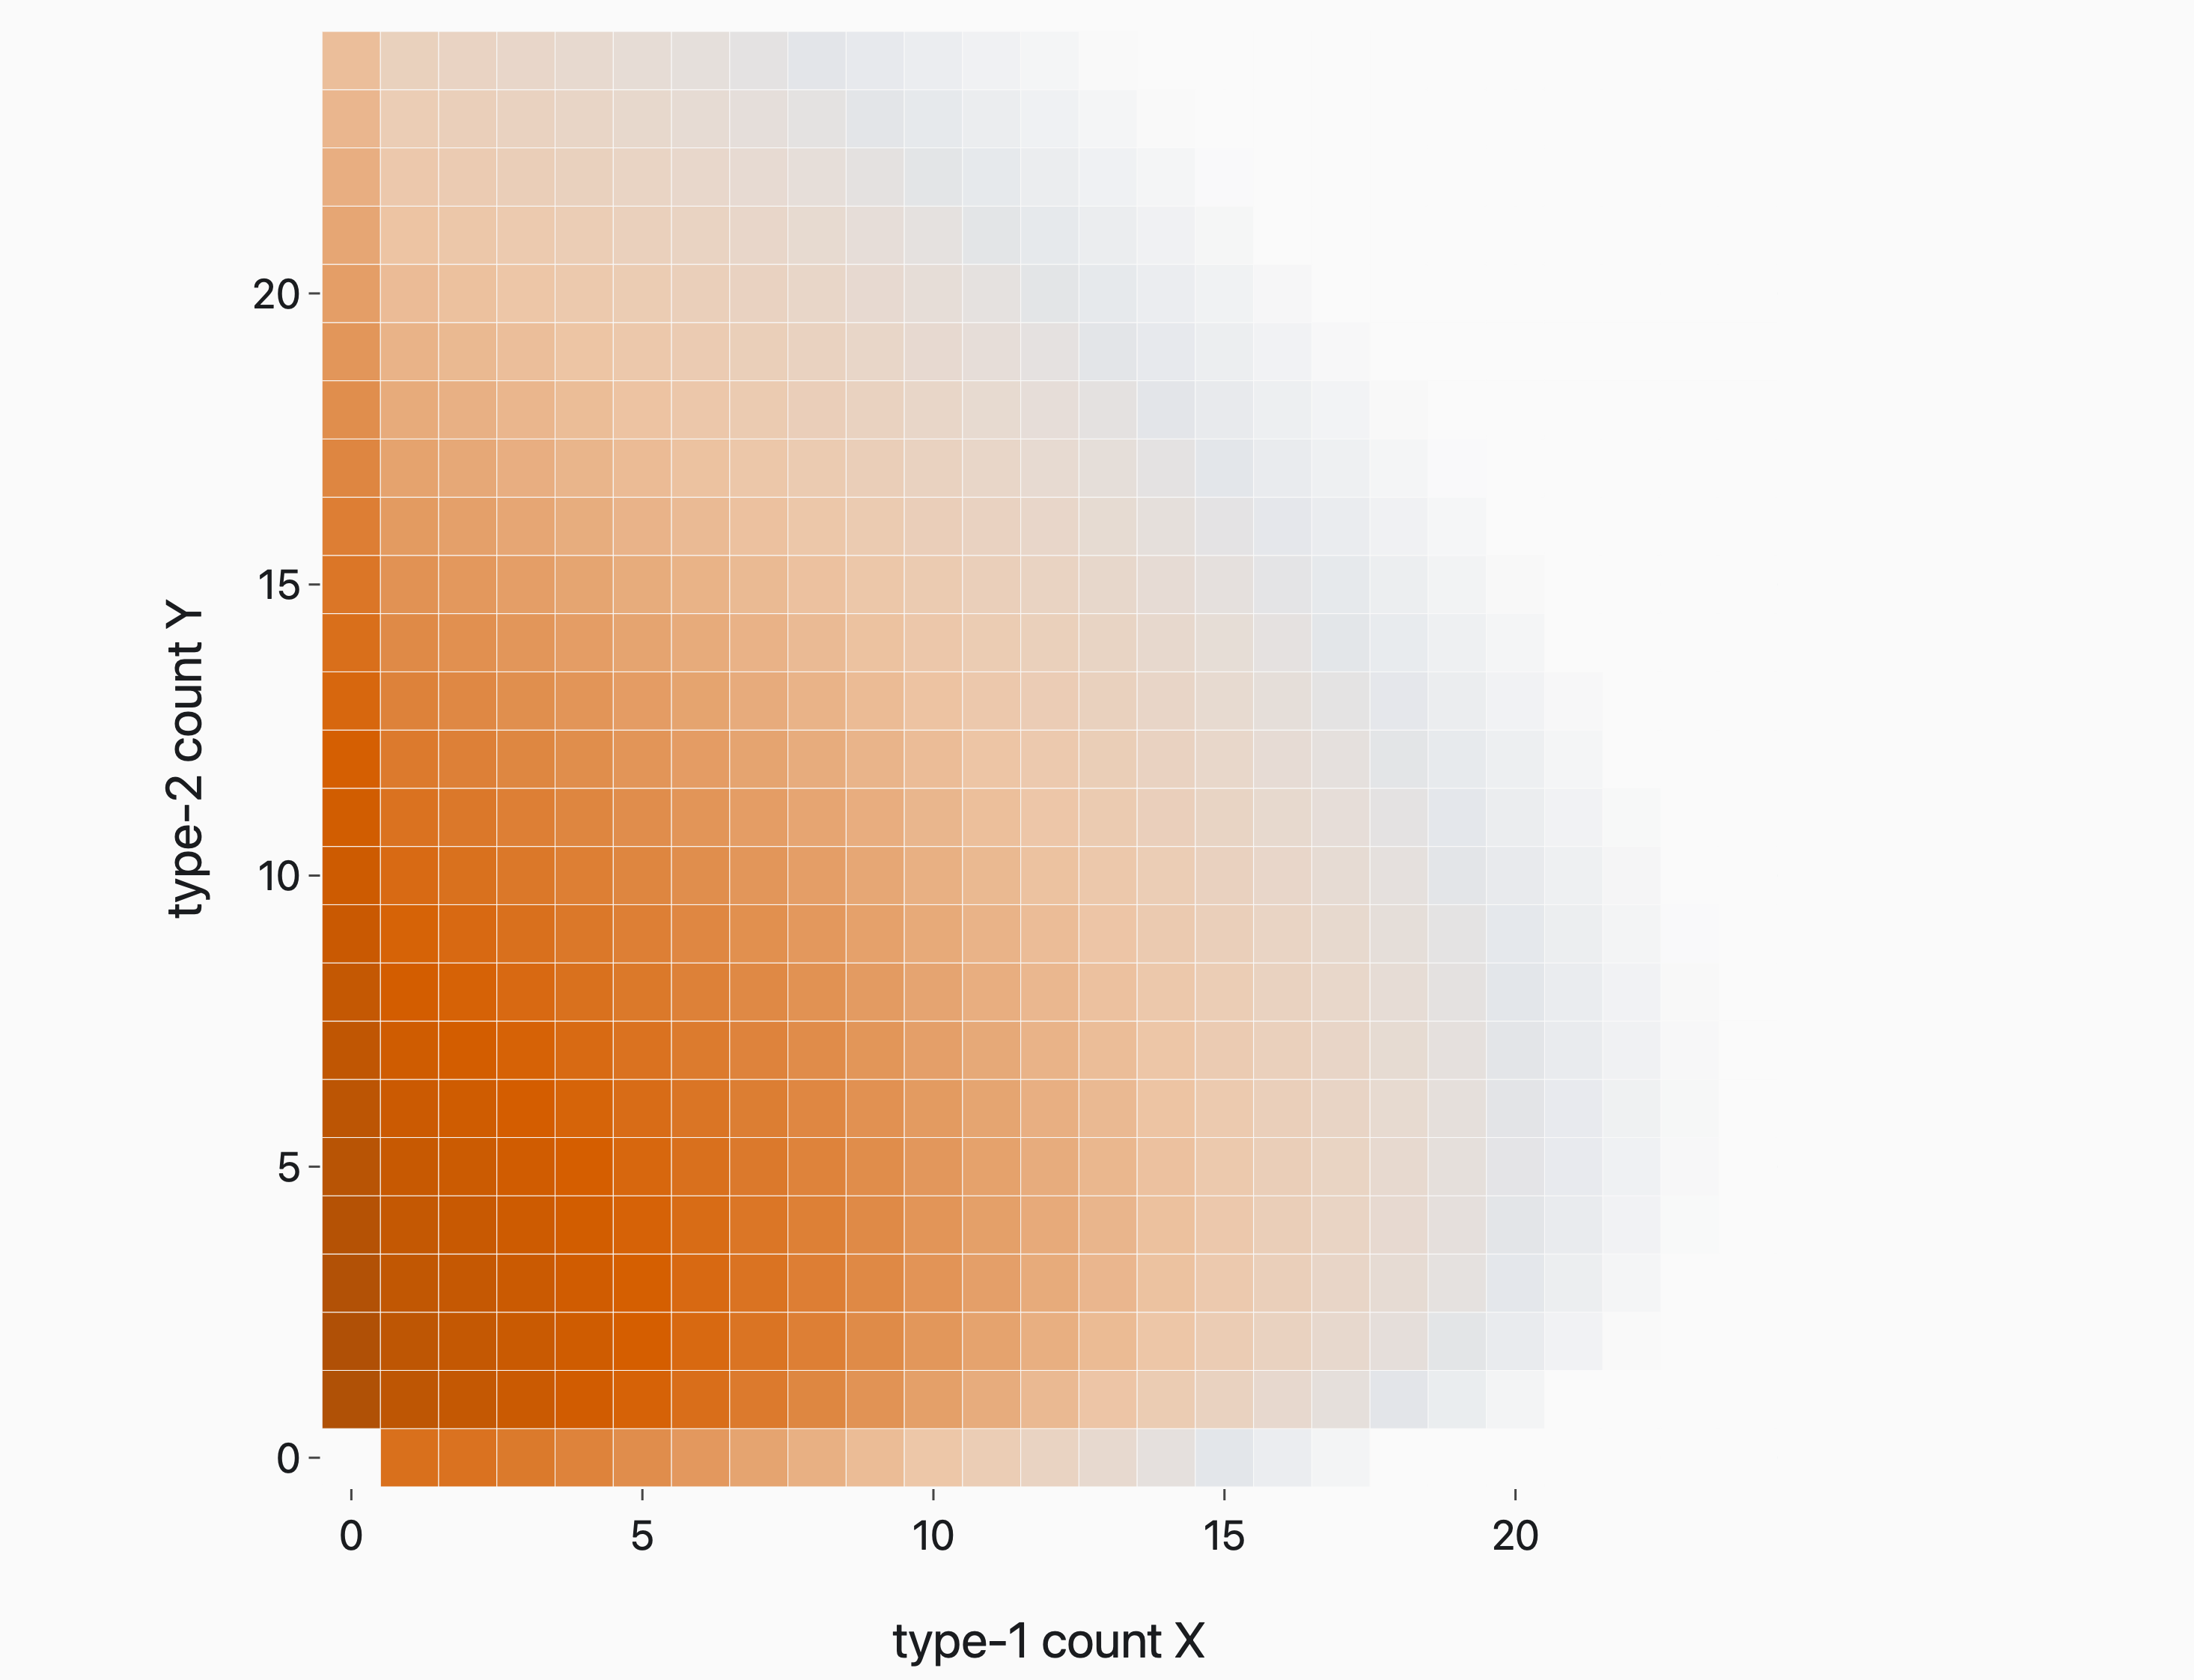
\includegraphics[width=\linewidth]{figures/fig_bdc_three_dists/panel_at_catastrophe.png}
    \caption{At catastrophe}
    \label{fig:dist-at-catastrophe}
  \end{subfigure}\hfill
  \begin{subfigure}[t]{0.32\textwidth}
    \centering
    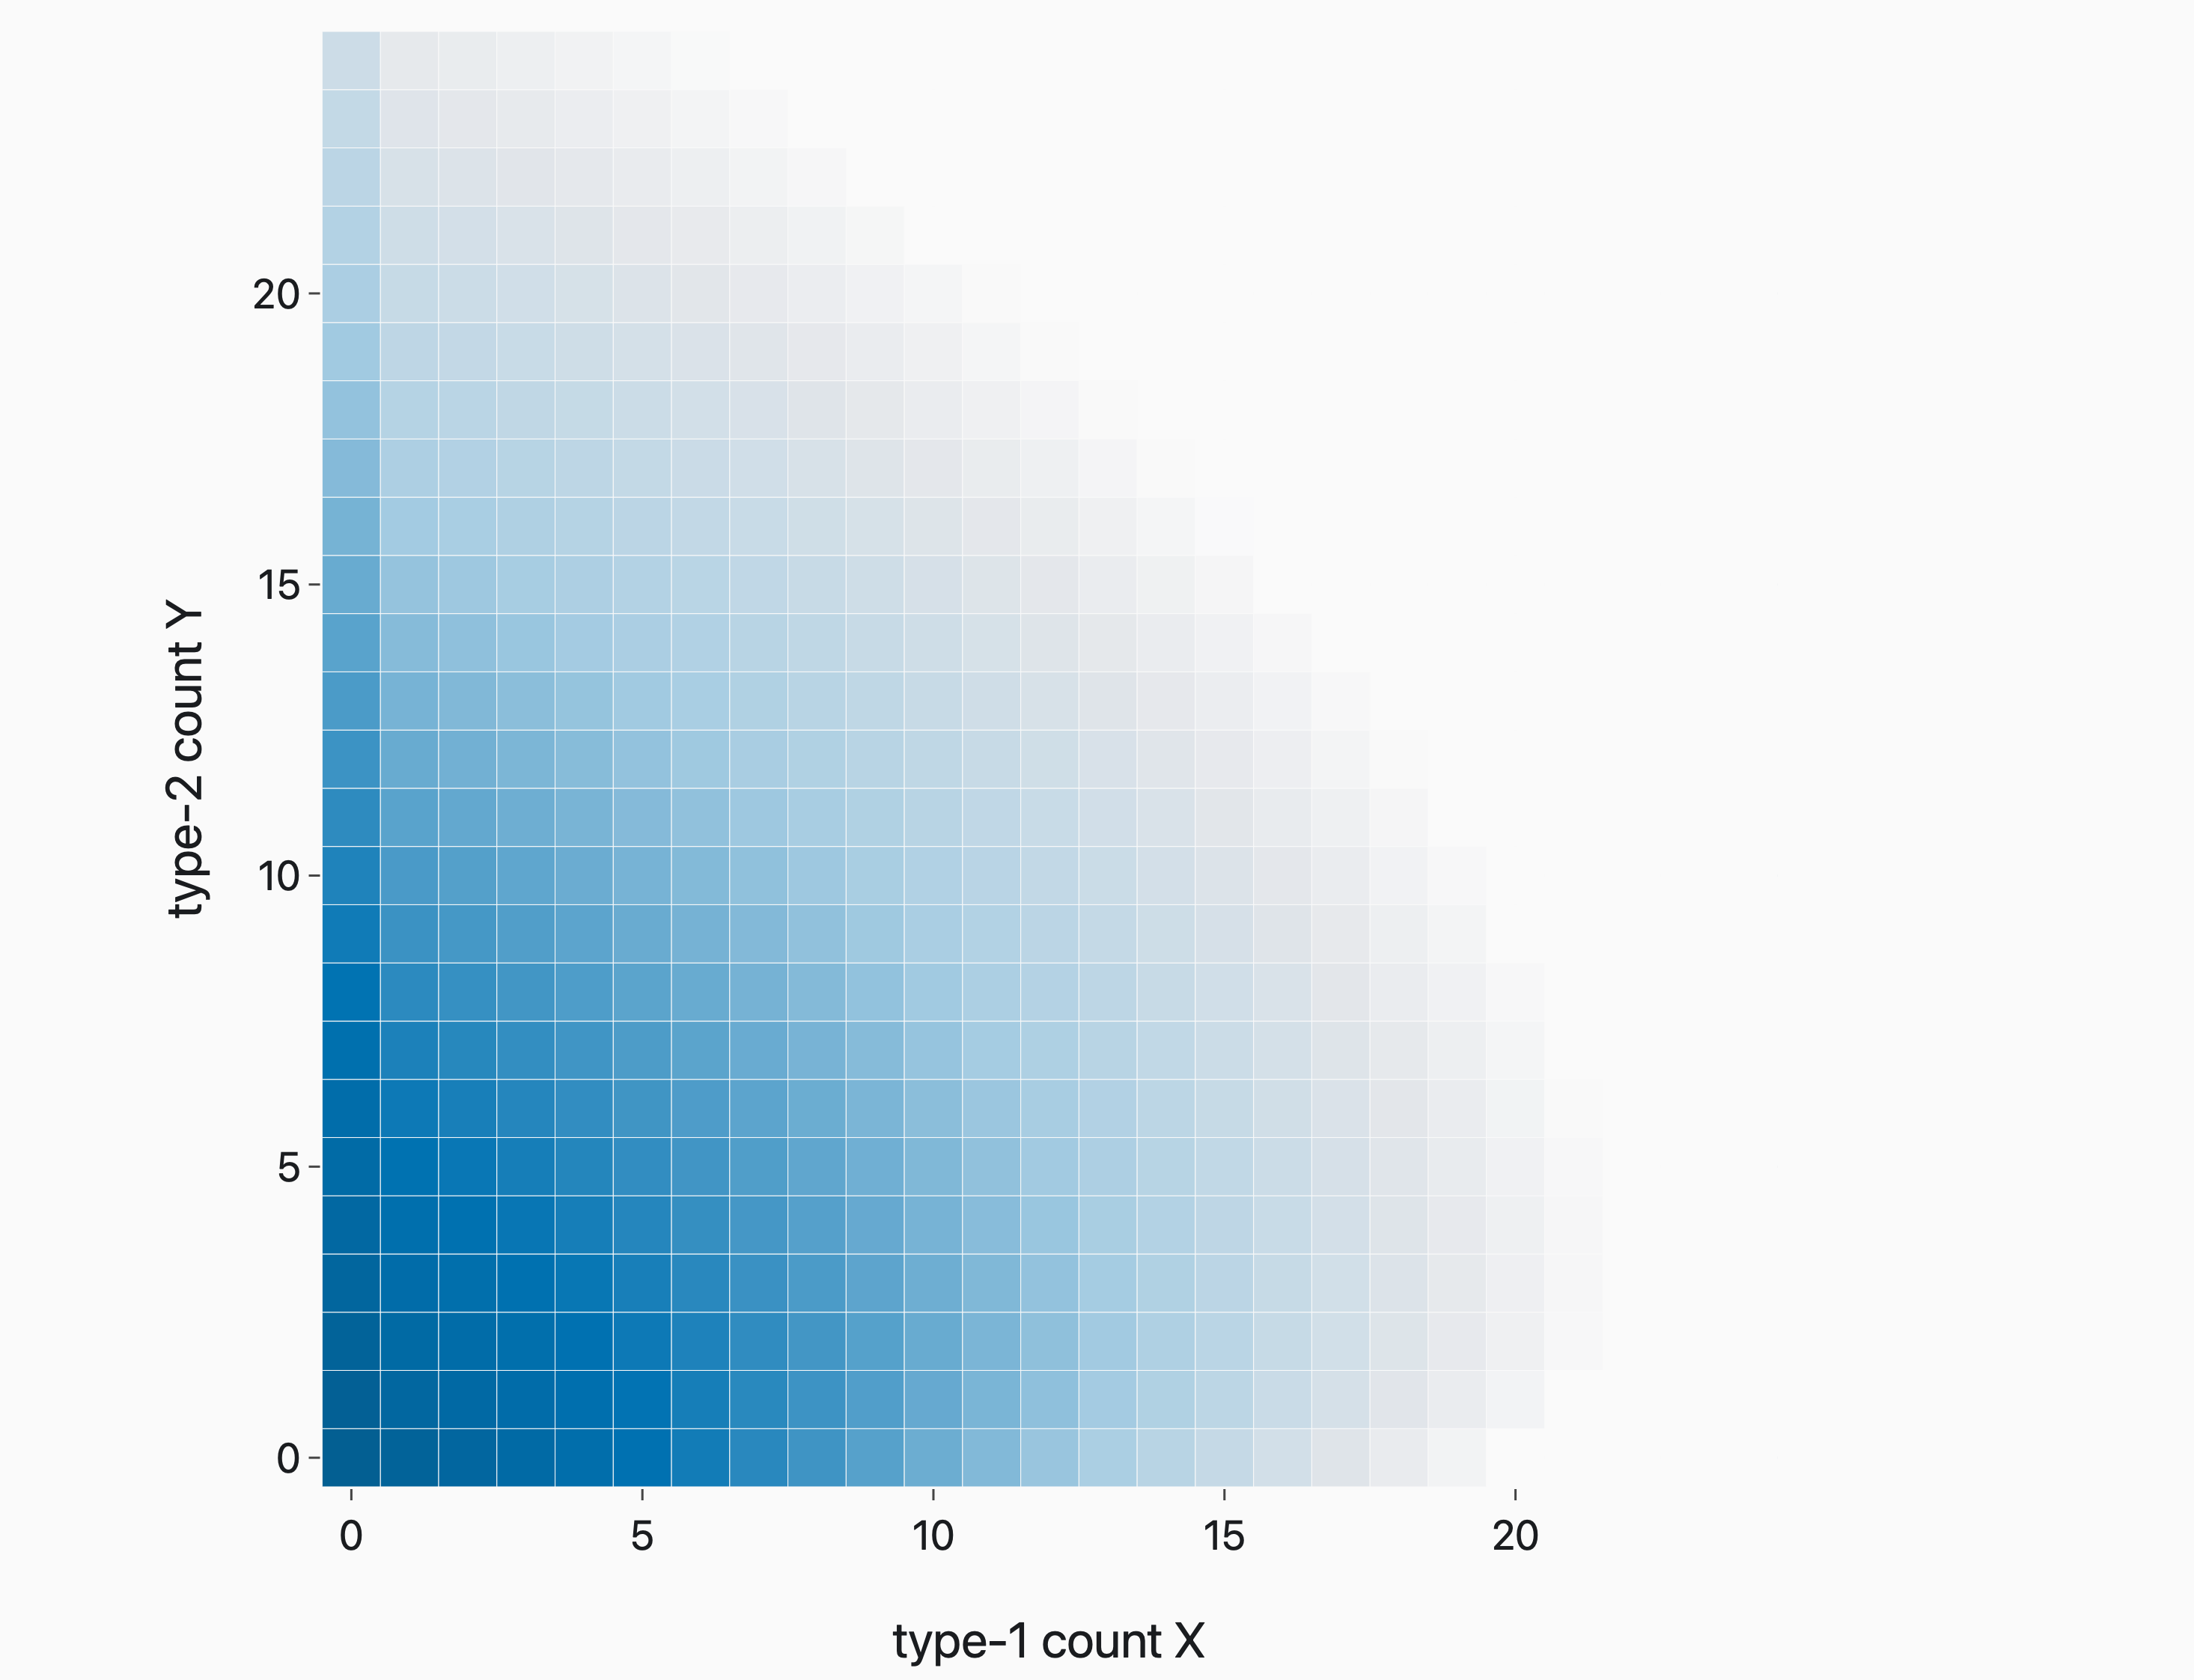
\includegraphics[width=\linewidth]{figures/fig_bdc_three_dists/panel_no_catastrophe.png}
    \caption{No catastrophe}
    \label{fig:dist-no-catastrophe}
  \end{subfigure}\hfill
  \begin{subfigure}[t]{0.32\textwidth}
    \centering
    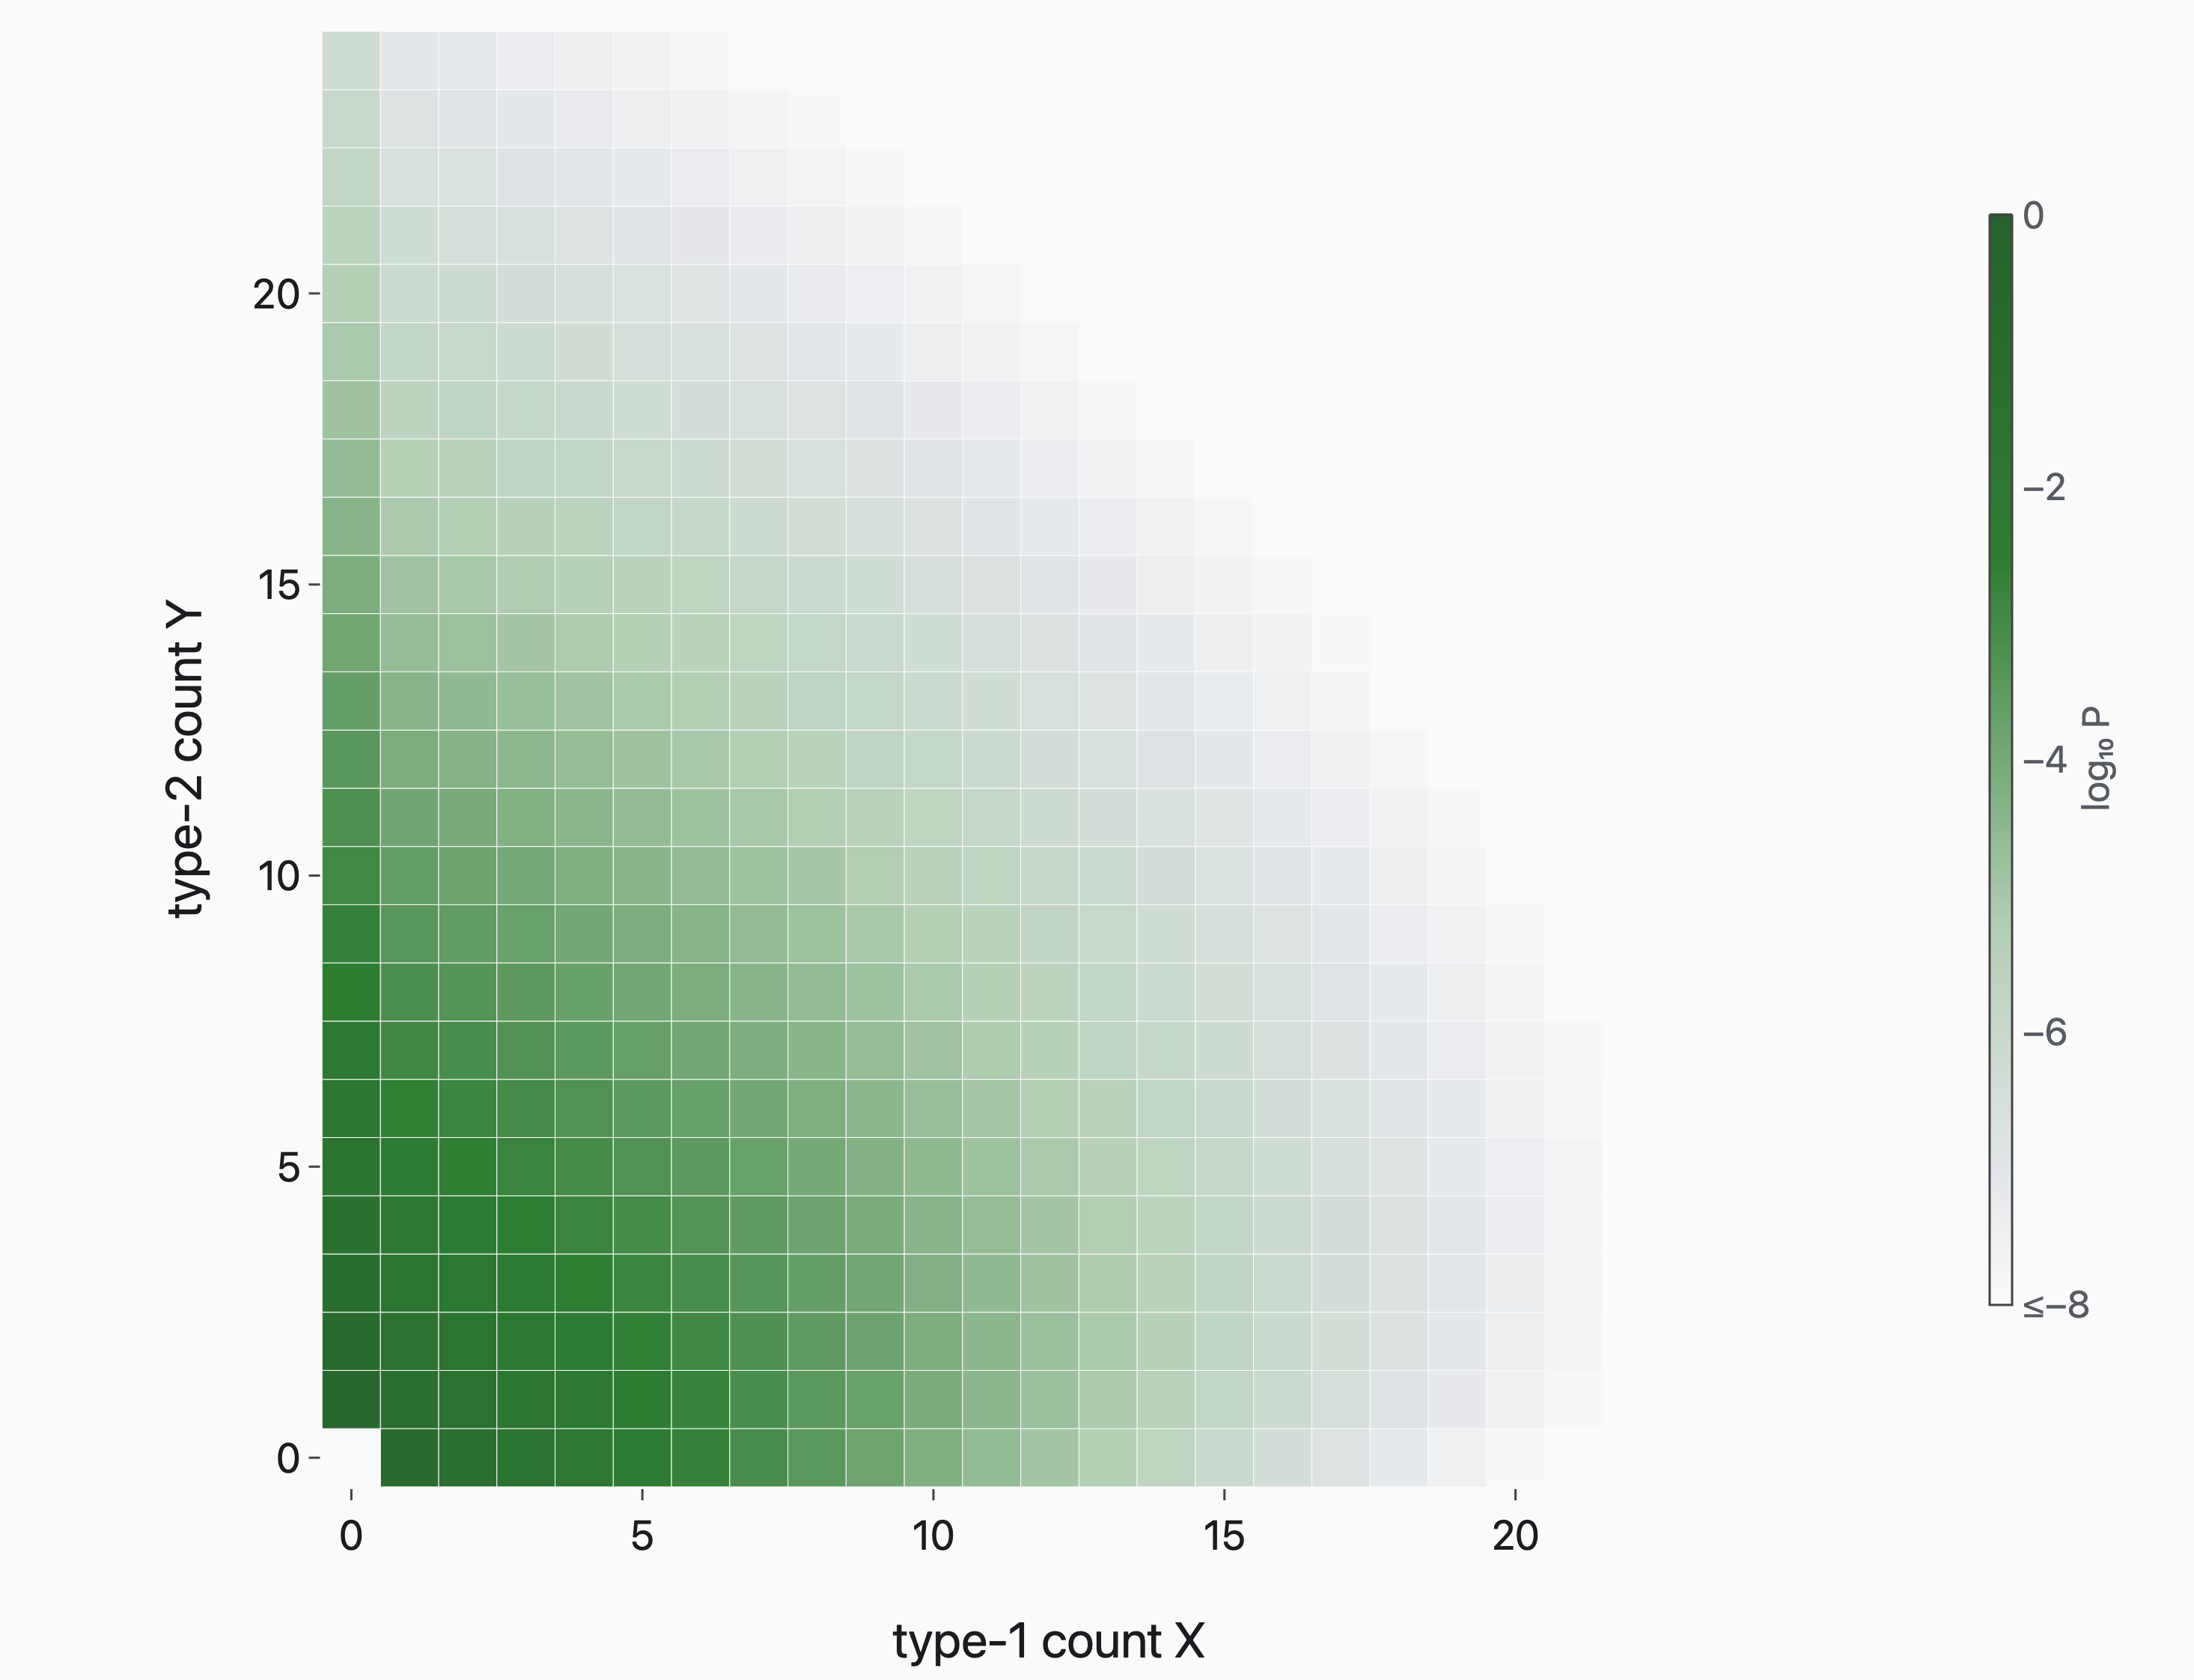
\includegraphics[width=\linewidth]{figures/fig_bdc_three_dists/panel_active.png}
    \caption{Active}
    \label{fig:dist-active}
  \end{subfigure}

  \caption{Three distributions encoded by the killed PGF at fixed time $t=3$, from one type-1 individual.
    (a)~Pre-catastrophe counts conditional on catastrophe at time $t$ (density sense).
    (b)~Counts conditional on no catastrophe up to $t$ (includes ordinary extinction at the origin).
    (c)~Active counts conditional on no catastrophe and non-extinction (log scale).
    Rates:
    $\lambda_1=0.75$, $\mu_1=0.3$, $\nu=0.7$, $\delta_1=0.001$,
    $\lambda_2=0.75$, $\mu_2=0.25$, $\delta_2=0.083$.
    Colour intensity scales are independent across panels.
    \explorerlink{https://files.volvox.site/users/pages/6a6852d29e3764e44c80325e/files/1785222034060-TT_bdc_distribution_visualiser.html}{Distribution visualiser}}
  \label{fig:three-pgf-distributions}
\end{figure}

\subsection{Ultimate release counts}
\label{sec:ultimate-release}

The three conditional laws above do not yet record the full unconditional law of the pre-catastrophe state, including paths that never release. Define the ultimate type-$1$ and type-$2$ release counts by
\begin{equation}
\label{eq:release-def}
(X_{\mathrm{rel}},Y_{\mathrm{rel}})
=
\begin{cases}
\bigl(X_{\tau_{\!c}-},\,Y_{\tau_{\!c}-}\bigr)
& \text{on }\{\tau_{\!c}<\infty\},\\[0.35em]
(0,0)
& \text{on }\{\tau_{\!c}=\infty\}.
\end{cases}
\end{equation}
Thus release is the left-limit population at the absorbing event when that event occurs, and is set to zero when no release event ever takes place.

\begin{remark}[Generic regime versus boundaries]
\label{rem:release-origin}
In the generic regime $\delta_1>0$, $\delta_2>0$, the only way to have $\tau_{\!c}=\infty$ is ordinary extinction to $(0,0)$ before the catastrophe clock fires. The origin atom of $(X_{\mathrm{rel}},Y_{\mathrm{rel}})$ is then exactly the forever-avoidance probability, and coincides with clearance without release. On certain catastrophe-rate boundaries (for instance $\delta_1=0$), paths with $\tau_{\!c}=\infty$ need not be extinct; \cref{eq:release-def} still assigns $(0,0)$ on those paths, now meaning ``no release event'' rather than ``empty burst''. The formulae below remain valid on those boundaries; only the biological reading of the origin atom changes.
\end{remark}

The joint law follows by integrating the catastrophe flux of \cref{sec:three-pgf-distributions}. For $m+n\ge 1$, the mass at $(m,n)$ is the integrated density of first entrance to $(\R,\R)$ from that pre-absorption state. The complementary forever-avoidance mass sits at the origin. Explicitly, with $\sigma_i(\infty)=\lim_{t\to\infty}\sigma_i(t)$ (so $\sigma_1(\infty)=h$ and $\sigma_2(\infty)=r_{2,-}$),
\begin{equation}
\label{eq:release-joint-pmf}
\Prob_i\{X_{\mathrm{rel}}=m,\,Y_{\mathrm{rel}}=n\}
=
\begin{cases}
\displaystyle
\sigma_i(\infty),
& (m,n)=(0,0),\\[1.0em]
\displaystyle
\int_0^\infty
(\delta_1 m+\delta_2 n)\,
p_{m,n}^{(i)}(t)\,
\dd t,
& m+n\ge 1.
\end{cases}
\end{equation}
These probabilities sum to one. The positive-support contribution equals
$\int_0^\infty\mathcal J_i(1,1,t)\,\dd t=\int_0^\infty\bigl(-\sigma_i'(t)\bigr)\,\dd t=1-\sigma_i(\infty)$,
since $\sigma_i(0)=1$ and $\sigma_i\downarrow\sigma_i(\infty)$.

The corresponding joint probability generating function is therefore
\begin{equation}
\boxed{
\begin{aligned}
\mathcal P_i^{\mathrm{rel}}(x,y)
&:=
\E_i\bigl[x^{X_{\mathrm{rel}}}y^{Y_{\mathrm{rel}}}\bigr]
\\
&=
\sigma_i(\infty)
+
\int_0^\infty
\mathcal J_i(x,y,t)\,
\dd t.
\end{aligned}
}
\label{eq:release-pgf}
\end{equation}
Coefficient extraction recovers \cref{eq:release-joint-pmf}: $\Prob_i\{X_{\mathrm{rel}}=m,Y_{\mathrm{rel}}=n\}=[x^my^n]\,\mathcal P_i^{\mathrm{rel}}(x,y)$.

When $\sigma_i(\infty)<1$, the law conditional on eventual catastrophe is supported on $\{(m,n):m+n\ge 1\}$ and has generating function
\begin{equation}
\label{eq:release-conditional}
\mathcal R_i^{\mathrm{cat}}(x,y)
:=
\E_i\bigl[
x^{X_{\mathrm{rel}}}y^{Y_{\mathrm{rel}}}
\bigm|
\tau_{\!c}<\infty
\bigr]
=
\frac{
\displaystyle
\int_0^\infty
\mathcal J_i(x,y,t)\,
\dd t
}{
1-\sigma_i(\infty)
}.
\end{equation}
This is the $T\to\infty$ limit of the horizon object $\mathcal R_{i,T}^{\mathrm{cat}}$ from \cref{sec:three-pgf-distributions}. The unconditional release PGF is the two-point mixture
\begin{equation}
\label{eq:release-mixture}
\mathcal P_i^{\mathrm{rel}}(x,y)
=
\sigma_i(\infty)\cdot 1
+
\bigl(1-\sigma_i(\infty)\bigr)\,
\mathcal R_i^{\mathrm{cat}}(x,y).
\end{equation}
For numerical evaluation, the joint masses in \cref{eq:release-joint-pmf} may be obtained by integrating the killed master equations on a truncated lattice and accumulating the catastrophe flux; \cref{fig:release-law} shows one such computation.

\begin{figure}[H]
  \centering
  % Shared image height so the (near-square) joint heatmap lines up with the wider
  % marginal bars.
  \begin{subfigure}[c]{0.40\textwidth}
    \centering
    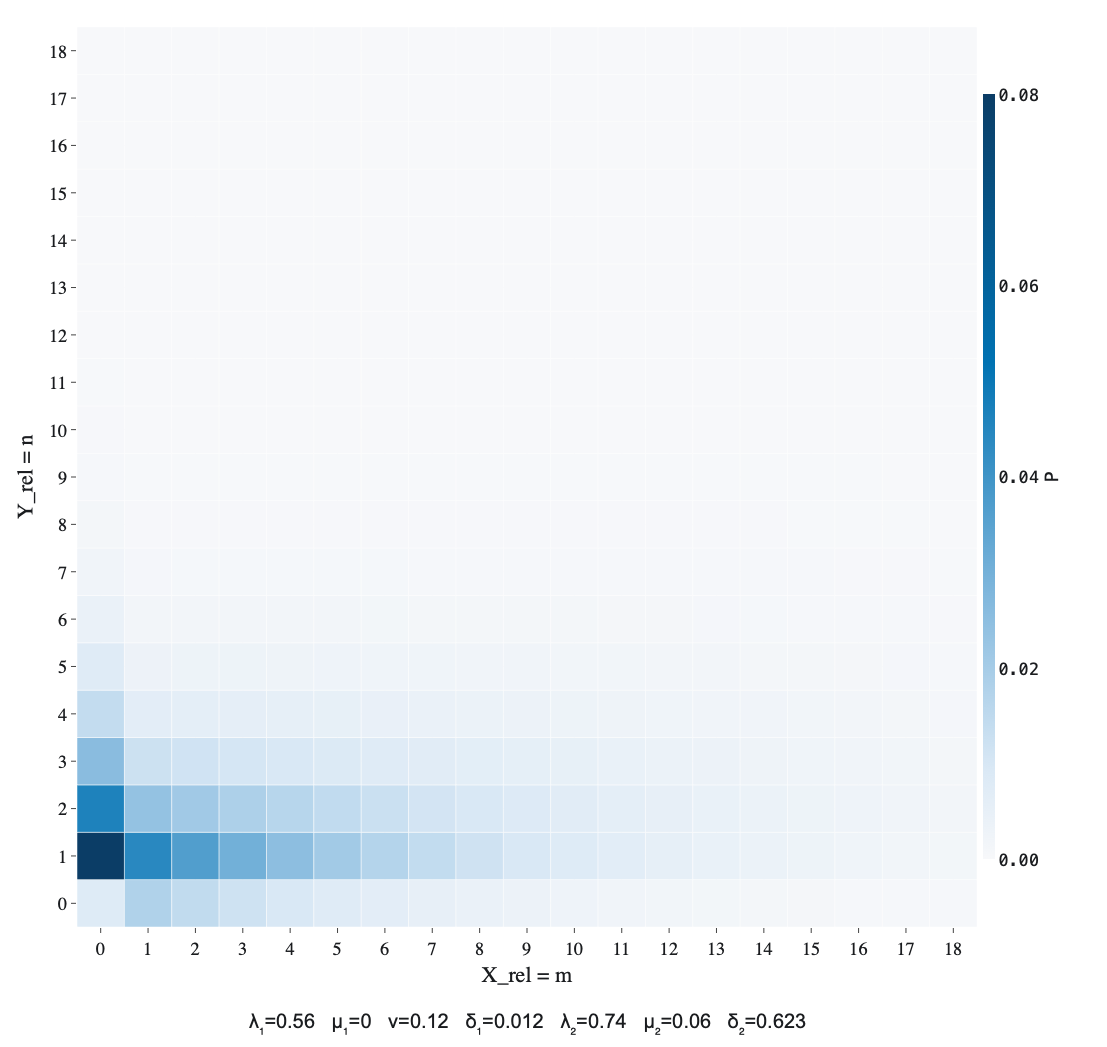
\includegraphics[height=5.2cm]{figures/fig_bdc_release/panel_joint.png}
    \caption{Joint law}
    \label{fig:release-joint}
  \end{subfigure}\hfill
  \begin{subfigure}[c]{0.56\textwidth}
    \centering
    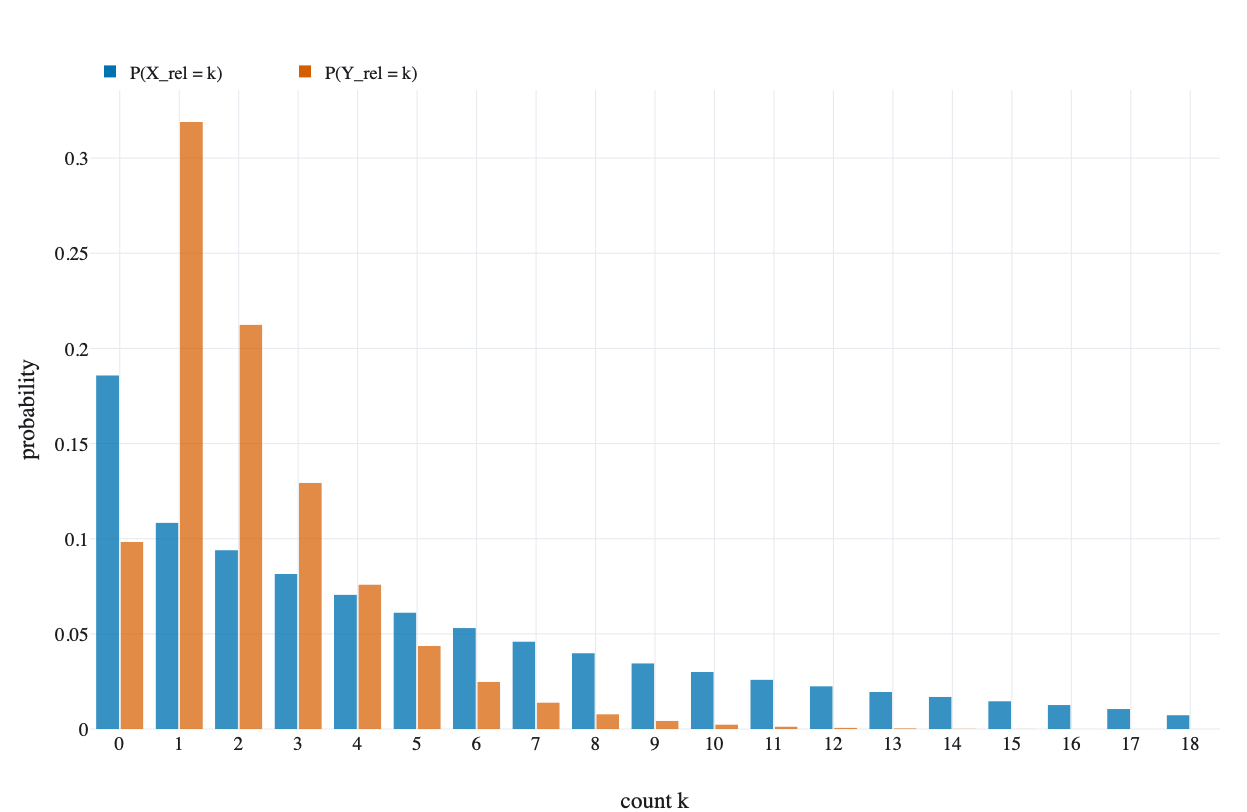
\includegraphics[height=5.2cm]{figures/fig_bdc_release/panel_marginals.png}
    \caption{Marginals}
    \label{fig:release-marginals}
  \end{subfigure}

  \caption{Unconditional ultimate release law $(X_{\mathrm{rel}},Y_{\mathrm{rel}})$ from one type-1 individual.
    (a)~Joint masses $\Prob_{(1,0)}\{X_{\mathrm{rel}}=m,\,Y_{\mathrm{rel}}=n\}$; the origin atom is forever-avoidance $\sigma_1(\infty)=h$ (clearance without release in the generic regime).
    (b)~Marginals $\Prob\{X_{\mathrm{rel}}=k\}$ (blue) and $\Prob\{Y_{\mathrm{rel}}=k\}$ (vermillion).
    Rates (on panel~(a)):
    $\lambda_1=0.56$, $\mu_1=0$, $\nu=0.12$, $\delta_1=0.012$,
    $\lambda_2=0.74$, $\mu_2=0.06$, $\delta_2=0.623$.
    Lattice truncation of the killed master equations; residual active mass at the numerical horizon is negligible.
    \explorerlink{https://files.volvox.site/users/pages/6a6852d29e3764e44c80325e/files/1785222143569-TT_bdc_release_visualiser.html}{Release visualiser}}
  \label{fig:release-law}
\end{figure}

The marginal generating functions are the specialisations $\mathcal P_i^{\mathrm{rel}}(x,1)$ and $\mathcal P_i^{\mathrm{rel}}(1,y)$. For $m\ge 1$,
\begin{equation}
\label{eq:release-marg-X}
\Prob_i\{X_{\mathrm{rel}}=m\}
=
\int_0^\infty
\sum_{n=0}^\infty
(\delta_1 m+\delta_2 n)\,
p_{m,n}^{(i)}(t)\,
\dd t,
\end{equation}
and for $n\ge 1$,
\begin{equation}
\label{eq:release-marg-Y}
\Prob_i\{Y_{\mathrm{rel}}=n\}
=
\int_0^\infty
\sum_{m=0}^\infty
(\delta_1 m+\delta_2 n)\,
p_{m,n}^{(i)}(t)\,
\dd t.
\end{equation}
Both marginals carry at least the origin atom $\sigma_i(\infty)$, but the event $\{X_{\mathrm{rel}}=0\}$ is strictly larger than $\{X_{\mathrm{rel}}=Y_{\mathrm{rel}}=0\}$ whenever catastrophe can occur from a pure type-$2$ state. Thus $\Prob_i\{X_{\mathrm{rel}}=0\}\ge\sigma_i(\infty)$, with equality if and only if pure type-$2$ states cannot trigger (in particular if $\delta_2=0$). The same remark applies to $Y_{\mathrm{rel}}$ with the roles of the types reversed.

Unconditional means $\E_i[X_{\mathrm{rel}}]$ and $\E_i[Y_{\mathrm{rel}}]$ are the first partial derivatives of $\mathcal P_i^{\mathrm{rel}}$ at $(1,1)$; conditional means given eventual catastrophe follow by dividing by $1-\sigma_i(\infty)$.
